%%%% IACR Transactions TEMPLATE %%%%
% This file shows how to use the iacrtrans class to write a paper.
% Written by Gaetan Leurent gaetan.leurent@inria.fr (2020)
% Public Domain (CC0)


%%%% 1. DOCUMENTCLASS %%%%
\documentclass[journal=tosc,final]{iacrtrans}
%%%% NOTES:
% - Change "journal=tosc" to "journal=tches" if needed
% - Change "submission" to "final" for final version
% - Add "spthm" for LNCS-like theorems


%%%% 2. PACKAGES %%%%
\usepackage{lipsum} % Example package -- can be removed
\usepackage{tikz}

%%%% 3. AUTHOR, INSTITUTE %%%%
\author{Jane Doe\inst{1,2} \and John Doe\inst{1}}
\institute{
  Institute A, City, Country, \email{jane@institute}
  \and
  Institute B, City, Country, \email{john@institute}
}
%%%% NOTES:
% - We need a city name for indexation purpose, even if it is redundant
%   (eg: University of Atlantis, Atlantis, Atlantis)
% - \inst{} can be omitted if there is a single institute,
%   or exactly one institute per author


%%%% 4. TITLE %%%%
\title{My New Paper}
%%%% NOTES:
% - If the title is too long, or includes special macro, please
%   provide a "running title" as optional argument: \title[Short]{Long}
% - You can provide an optional subtitle with \subtitle.

\begin{document}

\maketitle


%%%% 5. KEYWORDS %%%%
\keywords{Something \and Something else}


%%%% 6. ABSTRACT %%%%
\begin{abstract}
  In this paper we prove that the One-Time-Pad has perfect security.

\end{abstract}


%%%% 7. PAPER CONTENT %%%%
\section{Introduction}

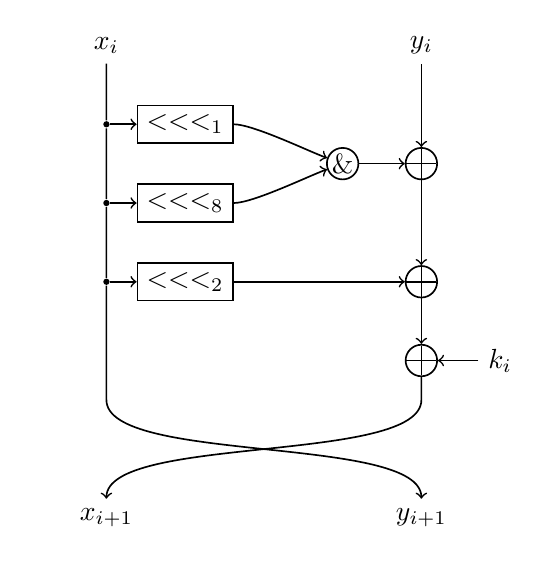
\begin{tikzpicture}
	[line width=0.6,trim left,
	box/.style = {
		draw
	},
	loosewire/.style = {
		looseness=0.5,
	},
	xor/.style = {
		draw, circle, inner sep=0cm, minimum size=0.4cm,
		append after command = {
			[shorten >=\pgflinewidth, shorten <=\pgflinewidth,]
			(\tikzlastnode.north) edge (\tikzlastnode.south)
			(\tikzlastnode.east) edge (\tikzlastnode.west)
		}
	},
	odot/.style = {
		draw, circle, inner sep=0cm, minimum size=0.4cm
	},
	dot/.style = {
		fill, circle, inner sep=0cm, minimum size=0.08cm
	},
	invisible/.style = {
		minimum size=0cm
	}]
	
	%Draw nodes
	\node at (1,7) (xin) {$x_i$};
	\node at (5,7) (yin) {$y_i$};
	\node[dot] at (1,6) (d1) {};
	\node[dot] at (1,5) (d2) {};
	\node[dot] at (1,4) (d3) {};
	\node[box] at (2,6) (S1) {$<<<_1$};
	\node[box] at (2,5) (S2) {$<<<_8$};
	\node[box] at (2,4) (S3) {$<<<_2$};
	\node[xor] at (5,5.5) (x1) {};
	\node[xor] at (5,4) (x2) {};
	\node[xor] at (5,3) (x3) {};
	\node[odot] at (4,5.5) (AND) {$\&$};
	\node at (6,3) (k) {$k_i$};
	\node at (1, 1) (xout) {$x_{i+1}$};
	\node at (5, 1) (yout) {$y_{i+1}$};
	\coordinate (cright) at (5, 2.5);
	\coordinate (cleft) at (1, 2.5);
	
	%Draw wires
	\draw[->] (d1) -- (S1);
	\draw[loosewire,->] (S1.east) to[out=0, in=160] (AND);
	\draw[->] (d2) -- (S2);
	\draw[loosewire,->] (S2.east) to[out=0, in=200] (AND);
	\draw[->] (AND) -- (x1);
	\draw[->] (d3) -- (S3);
	\draw[->] (S3.east) -- (x2);
	\draw[loosewire,->] (xin) -- (d1) -- (d2) -- (d3)
	-- (cleft) to[out=270, in=90] (yout.north);
	\draw[->] (yin) -- (x1);
	\draw[->] (x1) -- (x2);
	\draw[->] (x2) -- (x3);
	\draw[loosewire,->] (x3) -- (cright) to[out=270, in=90] (xout.north);
	\draw[->] (k.west) -- (x3);
\end{tikzpicture}%

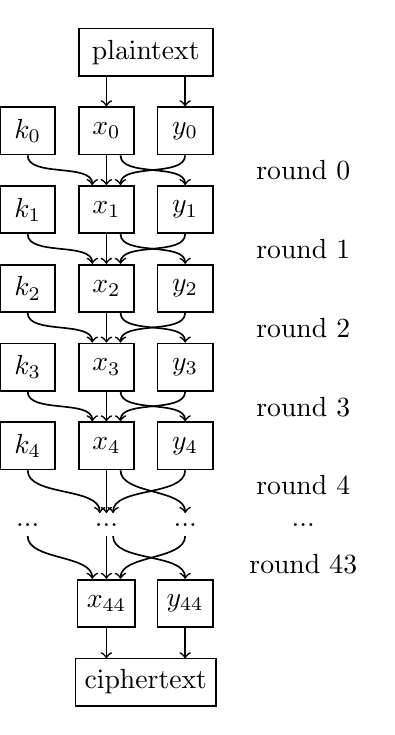
\begin{tikzpicture}
	[line width=0.6,trim left,
	box/.style = {
		draw,
		minimum height = 0.6cm,
		minimum width = 0.7cm
	},
	bigbox/.style = {
		draw,
		minimum height = 0.6cm,
		minimum width = 1.7cm
	},
	keybox/.style = {
		draw,
		minimum height = 3.6cm,
		minimum width = 0.7cm
	},
	nobox/.style = {
		minimum width = 0.7cm
	},
	wire/.style = {
		looseness=0.8,
		out=270,
		in=90
	},
	xor/.style = {
		draw, circle, inner sep=0cm, minimum size=0.4cm,
		append after command = {
			[shorten >=\pgflinewidth, shorten <=\pgflinewidth,]
			(\tikzlastnode.north) edge (\tikzlastnode.south)
			(\tikzlastnode.east) edge (\tikzlastnode.west)
		}
	},
	odot/.style = {
		draw, circle, inner sep=0cm, minimum size=0.4cm
	},
	dot/.style = {
		fill, circle, inner sep=0cm, minimum size=0.08cm
	},
	invisible/.style = {
		minimum size=0cm
	}]
	
	
	%Draw nodes
	\node[bigbox] at (1.5,7) (pt) {plaintext};
	\node[keybox] at (-1, 4.5) (key) {$K$};
	\node[box] at (1,6) (x0) {$x_0$};
	\node[box] at (2,6) (y0) {$y_0$};
	\node[box] at (0,6) (k0) {$k_0$};
	
	\node[box] at (1,5) (x1) {$x_1$};
	\node[box] at (2,5) (y1) {$y_1$};
	\node[box] at (0,5) (k1) {$k_1$};
	
	\node[box] at (1,4) (x2) {$x_2$};
	\node[box] at (2,4) (y2) {$y_2$};
	\node[box] at (0,4) (k2) {$k_2$};
	
	\node[box] at (1,3) (x3) {$x_3$};
	\node[box] at (2,3) (y3) {$y_3$};
	\node[box] at (0,3) (k3) {$k_3$};
	
	\node[box] at (1,2) (x4) {$x_4$};
	\node[box] at (2,2) (y4) {$y_4$};
	\node[box] at (0,2) (k4) {$k_4$};
	
	\node[nobox] at (1,1) (x5) {$...$};
	\node[nobox] at (2,1) (y5) {$...$};
	\node[nobox] at (0,1) (k5) {$...$};
	
	
	\node[box] at (1,0) (x44) {$x_{44}$};
	\node[box] at (2,0) (y44) {$y_{44}$};
	\node[bigbox] at (1.5,-1) (ct) {ciphertext};
	
	\coordinate(pt1) at (1,6.7);
	\coordinate(pt2) at (2,6.7);
	\coordinate(ct1) at (1,-0.7);
	\coordinate(ct2) at (2,-0.7);
	
	\coordinate(K0) at (-0.65,6);
	\coordinate(K1) at (-0.65,5);
	\coordinate(K2) at (-0.65,4);
	\coordinate(K3) at (-0.65,3);
	
	\node[nobox] at (3.5,5.5) {round 0};
	\node[nobox] at (3.5,4.5) {round 1};
	\node[nobox] at (3.5,3.5) {round 2};
	\node[nobox] at (3.5,2.5) {round 3};
	\node[nobox] at (3.5,1.5) {round 4};
	\node[nobox] at (3.5,1) {$...$};
	\node[nobox] at (3.5,0.5) {round 43};
	
	%Draw wires
	
	\draw[wire,->] (pt1) to (x0);
	\draw[wire,->] (pt2) to (y0);
	
	\draw[wire,->] (K0) to[out=0, in=180] (k0.180);
	\draw[wire,->] (K1) to[out=0, in=180] (k1.180);
	\draw[wire,->] (K2) to[out=0, in=180] (k2.180);
	\draw[wire,->] (K3) to[out=0, in=180] (k3.180);
	
	\draw[wire,->] (x0.300) to (y1.90);
	\draw[wire,->] (x0.270) to (x1.90);
	\draw[wire,->] (y0.270) to (x1.60);
	\draw[wire,->] (k0.270) to (x1.120);
	
	\draw[wire,->] (x1.300) to (y2.90);
	\draw[wire,->] (x1.270) to (x2.90);
	\draw[wire,->] (y1.270) to (x2.60);
	\draw[wire,->] (k1.270) to (x2.120);
	
	\draw[wire,->] (x2.300) to (y3.90);
	\draw[wire,->] (x2.270) to (x3.90);
	\draw[wire,->] (y2.270) to (x3.60);
	\draw[wire,->] (k2.270) to (x3.120);
	
	\draw[wire,->] (x3.300) to (y4.90);
	\draw[wire,->] (x3.270) to (x4.90);
	\draw[wire,->] (y3.270) to (x4.60);
	\draw[wire,->] (k3.270) to (x4.120);

	\draw[wire,->] (x4.300) to (y5.90);
	\draw[wire,->] (x4.270) to (x5.90);
	\draw[wire,->] (y4.270) to (x5.60);
	\draw[wire,->] (k4.270) to (x5.120);
	
	\draw[wire,->] (x5.300) to (y44.90);
	\draw[wire,->] (x5.270) to (x44.90);
	\draw[wire,->] (y5.270) to (x44.60);
	\draw[wire,->] (k5.270) to (x44.120);
	
	\draw[wire,->] (x44) to (ct1);
	\draw[wire,->] (y44) to (ct2);
	
\end{tikzpicture} 

A CPA was performed on the first 4 rounds of Simon-64/128. Each round brings in a 32-bit round key. The round keys $k_0, k_1, k_2$ and $k_3$ form the complete 128-bit key. 
For each round, the attack was split into 4 parts to extract the key bytewise.
Guessing 8 bits at once reduces the probability of wrongly guessed bits while the attack remains efficient.

The Hamming weight model was used for the power analysis. For each attacked round $i$, the internal state $x_{i+1}$ was chosen as an attack point.
$x_{i+1}$ depends on the 3 words $x_i$, $y_i$ and $k_i$ (see Figure xxx).

The round key $k_i$ is brought in with an XOR-operation. This makes it easy to split the attack into smaller parts because every bit of $k_i$ only influences 1 bit of $x_{i+1}$.

\subsubsection{Attack Steps}
The CPA attack was executed according to the following procedure:
\begin{enumerate}
	\item Collect $n$ power traces of length $m$. The whole measurement is a tuple $(T, P, C)$.
	
	$T$ is a Matrix of size $(n,m)$ which contains all traces $t_i$. $P$ contain the plaintexts $p_i$ and $C$ contains the ciphertexts $c_i$.
	$$T = 
	\begin{pmatrix}
		t_1 \\
		\vdots\\
		t_n
	\end{pmatrix}
	=
	\begin{pmatrix}
		t_{1,1}& \cdots& t_{1,m} \\
		\vdots & & \vdots \\
		t_{n,1}& \cdots& t_{n,m} \\
	\end{pmatrix}	
	\quad P = 	\begin{pmatrix}
		p_1 \\
		\vdots\\
		p_n
	\end{pmatrix}
	\quad C = 	\begin{pmatrix}
		c_1 \\
		\vdots\\
		c_n
	\end{pmatrix}
	$$

	\item Create key candidates $K^*$ and a bitmask $B$. In the first iteration of the attack, the values are defined like this:
	$$K^*=(k^*_0, ..., k^*_{255})=(0,...,255) \quad B = 255$$
	In later iterations, create key candidates based on key candidates that were marked as promising before. Adjust $B$ to mask all bits of the key which are guessed.
	
	\item For each combination of a key candidate and a plaintext, calculate the attacked intermediate state $x$. Apply the mask $B$ on $x$ by using a bitwise And-operation. Calculate the hamming weight $hw$ of the masked value. The resulting matrix $HW$ has the size $(n,256)$.
	$$
	HW =
	\begin{pmatrix}
		hw_{1,0}& \cdots& hw_{1,255} \\
		\vdots & & \vdots \\
		t_{n,0}& \cdots& t_{n,255} \\
	\end{pmatrix}
	$$
	
	\item Calculate the Pearson Correlation coefficient between every column of $T$ and every column of $HW$. The results is a matrix $\rho$ with size $(256, m)$. Compute $\hat{\rho}$ by selecting the the element with the largest absolute value in each row.
	$$
	\rho = 
	\begin{pmatrix}
		\rho_{0,1}& \cdots& \rho_{0,m} \\
		\vdots & & \vdots \\
		\rho_{255,1}& \cdots& \rho_{255,m} \\
	\end{pmatrix}	
	\quad
	\hat{\rho} = 
	\begin{pmatrix}
		\hat{\rho}_{0}\\
		\vdots \\
		\hat{\rho}_{255}\\
	\end{pmatrix}	
	$$
	\item From all elements $\hat{\rho}_i$, select the one with the largest absolute value. This value is denoted as $\tilde{\rho}$.
	\item Mark all elements $\hat{\rho}_i$ where its absolute value is closer to $\tilde{\rho}$ than some threshold $\tau$. For each marked value $\hat{\rho}_i$, the corresponding key candidate $k^*$ is classified as promising.
	\item Repeat the process from step 2 to extend the number of guessed bits.
	\item When all bits have been guessed, go through all promising key candidates and check if any plaintext $p_i$ results in the corresponding ciphertext $c_i$
	
	
	
\end{enumerate}





\section{Countermeausure}
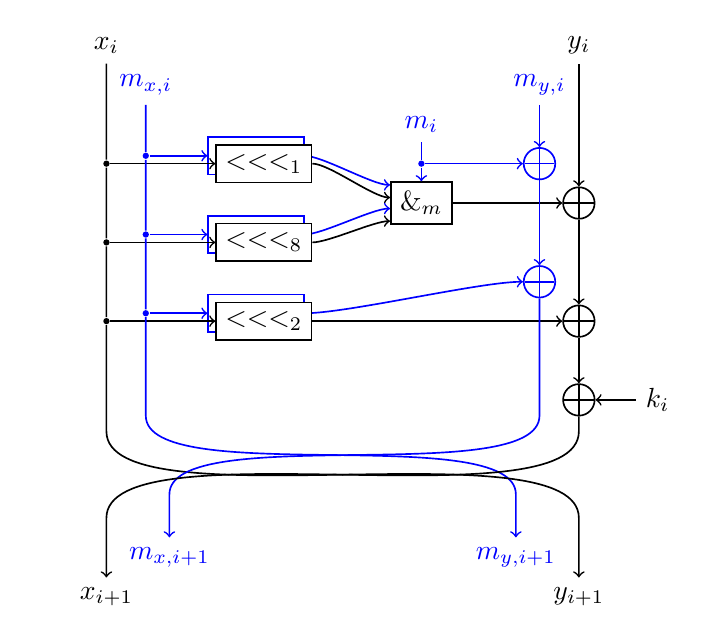
\begin{tikzpicture}
	[line width=0.6,trim left,
	box/.style = {
		draw,
		fill=white
	},
	loosewire/.style = {
		looseness=0.5,
	},
	xor/.style = {
		draw, circle, inner sep=0cm, minimum size=0.4cm,
		append after command = {
			[shorten >=\pgflinewidth, shorten <=\pgflinewidth,]
			(\tikzlastnode.north) edge (\tikzlastnode.south)
			(\tikzlastnode.east) edge (\tikzlastnode.west)
		}
	},
	xorblue/.style = {
		draw=blue, circle, inner sep=0cm, minimum size=0.4cm,
		append after command = {
			[shorten >=\pgflinewidth, shorten <=\pgflinewidth,]
			(\tikzlastnode.north) edge[draw=blue] (\tikzlastnode.south)
			(\tikzlastnode.east) edge[draw=blue] (\tikzlastnode.west)
		}
	},
	circ/.style = {
		draw, circle, inner sep=0cm, minimum size=0.4cm
	},
	dot/.style = {
		fill, circle, inner sep=0cm, minimum size=0.08cm
	}]
	
	%Draw nodes
	\node at (1,7.5) (xin) {$x_i$};
	\node[text=blue] at (1.5,7) (mx) {$m_{x,i}$};
	\node at (7,7.5) (yin) {$y_i$};
	\node[text=blue] at (6.5,7) (my) {$m_{y,i}$};
	\node[text=blue] at (5,6.5) (mi) {$m_i$};
	
	\node[dot,fill=blue] at (1.5,6.1) (d1m) {};
	\node[dot] at (1,6) (d1) {};
	\node[dot,fill=blue] at (1.5,5.1) (d2m) {};
	\node[dot] at (1,5) (d2) {};
	\node[dot,fill=blue] at (1.5,4.1) (d3m) {};
	\node[dot] at (1,4) (d3) {};
	
	\node[dot,fill=blue] at (5,6) (d4m) {};
	
	\node[box, draw=blue] at (2.9,6.1) (S1m) {$<<<_1$};
	\node[box] at (3,6) (S1) {$<<<_1$};
	\node[box, draw=blue] at (2.9,5.1) (S2m) {$<<<_8$};
	\node[box] at (3,5) (S2) {$<<<_8$};
	\node[box, draw=blue] at (2.9,4.1) (S3m) {$<<<_2$};
	\node[box] at (3,4) (S3) {$<<<_2$};
	
	\node[xorblue] at (6.5,6) (x1m) {};
	\node[xor] at (7,5.5) (x1) {};
	\node[xorblue] at (6.5,4.5) (x2m) {};
	\node[xor] at (7,4) (x2) {};
	\node[xor] at (7,3) (x3) {};
	
	\node[box] at (5,5.5) (AND) {$\&_m$};
	\node at (8,3) (k) {$k_i$};
	
	\node at (1, 0.5) (xout) {$x_{i+1}$};
	\node[text=blue] at (1.8, 1) (mxout) {$m_{x,i+1}$};
	
	\node at (7, 0.5) (yout) {$y_{i+1}$};
	\node[text=blue] at (6.2, 1) (myout) {$m_{y,i+1}$};
	
	\coordinate (cright) at (7, 2.6);
	\coordinate (cleft) at (1, 2.6);
	\coordinate (cright2) at (7, 1.5);
	\coordinate (cleft2) at (1, 1.5);
	\coordinate (crightm) at (6.5, 2.8);
	\coordinate (cleftm) at (1.5, 2.8);
	\coordinate (crightm2) at (6.2, 1.8);
	\coordinate (cleftm2) at (1.8, 1.8);
	
	%Draw wires
	\draw[->,draw=blue] (d1m) -- (S1m);
	\draw[->] (d1) -- (S1);
	
	\draw[loosewire,->,draw=blue] (S1m.east) to[out=0, in=180] (AND.150);
	\draw[loosewire,->] (S1.east) to[out=0, in=180] (AND.170);
	\draw[->,draw=blue] (d2m) -- (S2m);
	\draw[->] (d2) -- (S2);
	
	\draw[loosewire,->,draw=blue] (S2m.east) to[out=0, in=180] (AND.190);
	\draw[loosewire,->] (S2.east) to[out=0, in=180] (AND.210);
	
	\draw[->] (AND) -- (x1);
	
	\draw[->,draw=blue] (d3m) -- (S3m);
	\draw[->] (d3) -- (S3);
	
	\draw[loosewire,->,draw=blue] (S3m.east) to[out=0,in=180] (x2m);
	\draw[->] (S3.east) -- (x2);
	
	\draw[loosewire,->,draw=blue] (mx) -- (d1m) -- (d2m) -- (d3m)
	-- (cleftm) to[out=270, in=90] (crightm2) -- (myout.north);
	\draw[loosewire,->] (xin) -- (d1) -- (d2) -- (d3)
	-- (cleft) to[out=270, in=90] (cright2) -- (yout.north);
	
	
	\draw[->,draw=blue] (my) -- (x1m);
	\draw[->] (yin) -- (x1);
	\draw[->,draw=blue] (x1m) -- (x2m);
	\draw[->] (x1) -- (x2);
	\draw[->] (x2) -- (x3);
	
	\draw[loosewire,->,draw=blue] (x2m) -- (crightm) to[out=270, in=90] (cleftm2) -- (mxout.north);
	\draw[loosewire,->] (x3) -- (cright) to[out=270, in=90] (cleft2) -- (xout.north);
	\draw[->] (k.west) -- (x3);
	
	%additional wires for mask
	\draw[->,draw=blue] (mi) -- (d4m) -- (AND);
	\draw[->,draw=blue] (d4m) -- (x1m.west);
	
	%draw black boxes again to show them in front of blue arrows
	\node[box] at (3,6) (S1) {$<<<_1$};
	\node[box] at (3,5) (S2) {$<<<_8$};
	\node[box] at (3,4) (S3) {$<<<_2$};
	
\end{tikzpicture} 



\label{sec:main}



%%%% 8. BILBIOGRAPHY %%%%
\bibliographystyle{alpha}
\bibliography{abbrev3,crypto,biblio}
%%%% NOTES
% - Download abbrev3.bib and crypto.bib from https://cryptobib.di.ens.fr/
% - Use bilbio.bib for additional references not in the cryptobib database.
%   If possible, take them from DBLP.

\end{document}
